\documentclass[12pt]{article}
\usepackage[left=1cm, right=1cm, top=2cm,bottom=1.5cm]{geometry} 

\usepackage[parfill]{parskip}
\usepackage[utf8]{inputenc}
\usepackage[T2A]{fontenc}
\usepackage[russian]{babel}
\usepackage{enumitem}
\usepackage[normalem]{ulem}
\usepackage{amsfonts, amsmath, amsthm, amssymb, mathtools}
\usepackage{tabularx}
\usepackage{hhline}

\usepackage{accents}
\usepackage{fancyhdr}
\pagestyle{fancy}
\renewcommand{\headrulewidth}{1.5pt}
\renewcommand{\footrulewidth}{1pt}

\usepackage{graphicx}
\usepackage[figurename=Рис.]{caption}
\usepackage{subcaption}
\usepackage{float}

%%Наименование папки откуда забирать изображения
\graphicspath{ {./images/} }

%%Изменение формата для ввода доказательства
\renewcommand{\proofname}{$\square$  \nopunct}
\renewcommand\qedsymbol{$\blacksquare$}

%%Изменение отступа на таблицах
\addto\captionsrussian{%
	\renewcommand{\proofname}{$\square$ \nopunct}%
}
%% Римские цифры
\newcommand{\RN}[1]{%
	\textup{\uppercase\expandafter{\romannumeral#1}}%
}

%% Для удобства записи
\newcommand{\MR}{\mathbb{R}}
\newcommand{\MQ}{\mathbb{Q}}
\newcommand{\MN}{\mathbb{N}}
\newcommand{\MTB}{\mathbb{T}}
\newcommand{\MI}{\mathrm{I}}
\newcommand{\MJ}{\mathrm{J}}
\newcommand{\MH}{\mathrm{H}}
\newcommand{\MT}{\mathrm{T}}
\newcommand{\MU}{\mathcal{U}}
\newcommand{\MV}{\mathcal{V}}
\newcommand{\MW}{\mathcal{W}}
\newcommand{\VN}{\varnothing}
\newcommand{\VE}{\varepsilon}

\theoremstyle{definition}
\newtheorem{defn}{Опр:}
\newtheorem{rem}{Rm:}
\newtheorem{prop}{Утв.}
\newtheorem{exrc}{Упр.}
\newtheorem{lemma}{Лемма}
\newtheorem{theorem}{Теорема}
\newtheorem{corollary}{Следствие}

\newenvironment{cusdefn}[1]
{\renewcommand\thedefn{#1}\defn}
{\enddefn}

\DeclareRobustCommand{\divby}{%
	\mathrel{\text{\vbox{\baselineskip.65ex\lineskiplimit0pt\hbox{.}\hbox{.}\hbox{.}}}}%
}
%Короткий минус
\DeclareMathSymbol{\SMN}{\mathbin}{AMSa}{"39}
%Длинная шапка
\newcommand{\overbar}[1]{\mkern 1.5mu\overline{\mkern-1.5mu#1\mkern-1.5mu}\mkern 1.5mu}
%Функция знака
\DeclareMathOperator{\sgn}{sgn}

%Функция ранга
\DeclareMathOperator{\rk}{\text{rk}}

%Обозначение константы
\DeclareMathOperator{\const}{\text{const}}

%Интеграл в большом формате
\DeclareMathOperator{\dint}{\displaystyle\int}
\newcommand{\ddint}[2]{\displaystyle\int\limits_{#1}^{#2}}

\newcommand{\smallerrel}[1]{\mathrel{\mathpalette\smallerrelaux{#1}}}
\newcommand{\smallerrelaux}[2]{\raisebox{.1ex}{\scalebox{.75}{$#1#2$}}}

\newcommand{\smallin}{\smallerrel{\in}}
\newcommand{\smallnotin}{\smallerrel{\notin}}

\newcommand*{\medcap}{\mathbin{\scalebox{1.25}{\ensuremath{\cap}}}}%
\newcommand*{\medcup}{\mathbin{\scalebox{1.25}{\ensuremath{\cup}}}}%

\makeatletter
\newcommand{\vast}{\bBigg@{3.5}}
\newcommand{\Vast}{\bBigg@{5}}
\makeatother

%Промежуточное значение для sup\inf, поскольку они имеют разную высоту
\newcommand{\newsup}{\mathop{\smash{\mathrm{sup}}}}
\newcommand{\newinf}{\mathop{\mathrm{inf}\vphantom{\mathrm{sup}}}}

%Скалярное произведение
\DeclarePairedDelimiterX{\inner}[2]{\langle}{\rangle}{#1, #2}

%Подпись символов снизу
\newcommand{\ubar}[1]{\underaccent{\bar}{#1}}

%% Шапка для букв сверху
\newcommand{\wte}[1]{\widetilde{#1}}

\begin{document}
\lhead{Математический анализ - \RN{2}}
\chead{Шапошников С.В.}
\rhead{Лекция - 26}

\section*{Формула замены переменных}

\begin{lemma}
	Пусть функция $\varphi$ на отрезке $[a,b]$ удовлетворяет условию Липшица:
	$$
		\forall x_1,x_2 \in [a,b], \, \exists \, M > 0 \colon |\varphi(x_1) - \varphi(x_2)| \leq M{\cdot}|x_1 - x_2|
	$$
	Тогда  $\forall$ множества $E \subset [a,b]$ меры ноль по Лебегу, его образ $\varphi(E)$ также будет множеством меры ноль.
\end{lemma}
\begin{proof}
	Рассмотрим интервал $\MI = (c - \delta, c + \delta)$ и его образ под действием функции $\varphi$. Можно сразу сказать, что из $c \in \MI \Rightarrow \varphi(c) \in \varphi(\MI)$. Если $y \in \varphi(\MI)$, то $\exists \, x \in \MI \colon y = \varphi(x)$. Измерим расстояние между $y$ и $\varphi(c)$:
	$$
		|y -\varphi(c)| = |\varphi(x) - \varphi(c)| \leq M{\cdot}|x-c| < M\delta
	$$
	где последнее неравенство верно в силу того, что $x \in \MI$. Таким образом, получаем: 
	$$
		\varphi(\MI) \subset \MJ = (\varphi(c) - M\delta, \varphi(c) + M\delta), \, |\MI| = 2\delta \Rightarrow |\MJ| = M{\cdot}|\MI| = 2M\delta
	$$
	Возьмем $E$ - множество меры ноль по Лебегу, тогда:
	$$
		\forall \VE > 0, \, \exists \, \MI_n \colon E \subset \bigcup\limits_n \MI_n \wedge \sum\limits_{n} |\MI_n| < \VE
	$$
	Следовательно, $\forall \, \MI_n$ мы можем подобрать интервалы $\MJ_n$ и рассмотреть образ множества меры ноль: 
	$$
		\varphi(\MI_n) \subset \MJ_n, \, |\MJ_n| = M{\cdot}|\MI_n| \Rightarrow \varphi(E) \subset \varphi\left(\bigcup\limits_n \MI_n\right) \subset \bigcup\limits_n \varphi(\MI_n) \subset \bigcup\limits_n \MJ_n
	$$
	где второе включение верно в силу следующего:
	$$
		y \in  \varphi\left(\bigcup\limits_n \MI_n\right) \Rightarrow \exists \, x \in \bigcup\limits_n \MI_n \colon \varphi(x) = y \Rightarrow \exists \, j \colon x \in \MI_j \Rightarrow y \in \varphi(\MI_j) \Rightarrow y \in \bigcup\limits_n \varphi(\MI_n)
	$$
	Заметим, что сумма длин $\MJ_n$ будет маленькой:
	$$
		\sum\limits_n |\MJ_n| = \sum\limits_n M{\cdot}|\MI_n| = M{\cdot}\!\sum\limits_n |\MI_n| < M{\cdot}\VE
	$$
	Поскольку $M > 0$ - константа, то значение в правой части можно сделать сколь угодно маленьким, следовательно, $\varphi(E)$ это множество меры ноль по Лебегу.
\end{proof}
\begin{rem}
	Для просто непрерывных функций утверждение выше - не верно. 
\end{rem}
\textbf{Пример}: Рассмотрим лестницу Кантора: $C(0) = 0, \, C(1) = 1$, далее на центральном выбрасываемом интервале $C(x) = \tfrac{1}{2}$, на следующих выбрасываемых интервалах $C(x) = \tfrac{1}{4}$ на левом промежутке и $C(x) = \tfrac{3}{4}$ на правом, и так далее. Получим монотонную функцию, определенную всюду вне Канторовского множества. Доопределяем её до непрерывной функции $C(x)$ на всем промежутке $[0,1]$, это и будет лестницей Кантора. Таким образом, $C(x)$ - непрерывная и не убывает на $[0,1]$, тогда рассмотрим следующую функцию:
$$
	f(x) = \dfrac{C(x) + x}{2} \colon [0,1] \to [0,1]
$$
Функция $f(x)$ - строго монотонна и является гомеоморфизмом. Что эта функция делает с дополнением множества Кантора $=C_A$? Отображает в интервалы, длина которых равна длине интервалов дополнения множества Кантора на коэффициент наклона:
$$
	f(C_A) = \bigcup\limits_n \MI_n \colon \sum\limits_{n} |\MI_n| = \dfrac{1}{2}{\cdot}1 = \dfrac{1}{2}
$$
Следовательно, множество Кантора $= A$ не может перейти в множество меры ноль $\Rightarrow f(A)$ - не является множеством меры ноль. Лестница Кантора - не Липшецева функция.

\begin{theorem}(\textbf{Формула замены переменных})
	Пусть $\varphi \colon [\alpha,\beta] \to [a,b]$ - диффеоморфизм (непрерывно дифференцируемая биекция и её обратная функция) и функция $f$ - интегрируема по Риману на $[a,b]$. Тогда функция $f\left(\varphi(t)\right){\cdot}|\varphi^\prime(t)|$ интегрируема на отрезке $[\alpha, \beta]$ и выполнено следующее:
	$$
		\ddint{\alpha}{\beta}f\left(\varphi(t)\right){\cdot}|\varphi^\prime(t)|dt = \ddint{a}{b}f(x)dx
	$$
\end{theorem}
\begin{rem}
	Модуль в функции не должен смущать, поскольку $\varphi$ - диффеоморфизм $\Rightarrow$ производная нигде не ноль, значит она везде либо $> 0$, либо $< 0$ и тем самым модуль раскрывается либо с плюсом, либо с минусом, но раскрытие модуля с минусом согласуется с обычной формулой, когда $\alpha$ и $\beta$ расставляем в другом порядке (или $a$ и $b$).
\end{rem}
\begin{proof}
	Пусть $E$ - множество точек разрыва функции $f$, по критерию Лебега $E$ - это множество меры ноль. Рассмотрим прообраз этого множества $\varphi^{-1}(E)$. $\varphi^{-1}$ - непрерывно дифференцируемая функция, производная ограничена поскольку она непрерывна на отрезке $\Rightarrow$ она Липшицева по теореме Лагранжа:
	$$
		\forall x_1, x_2 \in [a,b], \, |\varphi^{-1}(x_1) - \varphi^{-1}(x_2)| = |(\varphi^{-1})^\prime(c)|{\cdot}|x_1 - x_2| \leq M{\cdot}|x_1 - x_2|, \, M = \max\limits_{x \smallin [a,b]}|(\varphi^{-1})^\prime(x)|
	$$
	Тогда образ множества меры ноль $\varphi^{-1}(E)$ это множество меры ноль на отрезке $[\alpha,\beta]$ по лемме выше. Пусть $t_0 \notin \varphi^{-1}(E)$, тогда $\varphi(t_0)$ - точка непрерывности функции $f$ и $f\left(\varphi(t)\right){\cdot}|\varphi^\prime(t)|$ непрерывна в $t_0$.
	Следовательно, $f\left(\varphi(t)\right){\cdot}|\varphi^\prime(t)|$ почти всюду непрерывна, $f$ - ограничена, а $\varphi$ - непрерывная функция на отрезке, то есть тоже ограничена $\Rightarrow$ по критерию Лебега $f\left(\varphi(t)\right){\cdot}|\varphi^\prime(t)|$ - интегрируема.
	
	Для доказательства равенства, рассмотрим Римановы суммы. Пусть $\varphi^\prime > 0$ (для $\varphi^\prime <0$ доказывается аналогично). Возьмем отрезок $[\alpha,\beta]$ и его любое разбиение $\MTB_t$, тогда:
	$$
		\sigma(f\left(\varphi(t)\right){\cdot}\varphi^\prime(t), \MTB_t,\xi) = \sum\limits_k f\left(\varphi(\xi_k)\right){\cdot}\varphi^\prime(\xi_k){\cdot}(t_k - t_{k-1})
	$$
	Выбираем $\xi_k$ таким образом, чтобы $\varphi^\prime(\xi_k){\cdot}(t_k - t_{k-1}) = \varphi(t_k) - \varphi(t_{k-1})$ по теореме Лагранжа. Тогда:
	$$
		\sum\limits_k f\left(\varphi(\xi_k)\right){\cdot}\varphi^\prime(\xi_k){\cdot}(t_k - t_{k-1}) = \sum\limits_k f\left(\varphi(\xi_k)\right){\cdot}\left(\varphi(t_k) - \varphi(t_{k-1})\right)
	$$
	Поскольку $\varphi^\prime > 0$, то $\varphi(t_k) > \varphi(t_{k-1})$ и точка $\varphi(\xi_k) \in [\varphi(t_{k-1}), \varphi(t_k)]$. Таким образом, мы получаем набор точек, которые формируют разбиение $\MTB_x$ отрезка $[a,b]$ и отмеченные точки $\varphi(\xi)$. Заметим, что:
	$$
		|\varphi(t_k) - \varphi(t_{k-1})| \leq \overline{M}{\cdot}|t_k - t_{k-1}|, \, \overline{M} = \max\limits_{x \smallin [\alpha,\beta]}|\varphi^\prime(x)| \Rightarrow \lambda(\MTB_t) \to 0 \Rightarrow \lambda(\MTB_x) \to 0
	$$
	Поскольку мы знаем, что интегралы существуют, то выбор отмеченных точек не важен ($\varphi(\xi)$ - не любые, но масштаб $\lambda(\MTB_x)$ стремится к нулю). Таким образом:
	$$
		\lim\limits_{\lambda(\MTB_t) \to 0}\sum\limits_k f\left(\varphi(\xi_k)\right){\cdot}\varphi^\prime(\xi_k){\cdot}(t_k - t_{k-1}) = \ddint{\alpha}{\beta}f\left(\varphi(t)\right){\cdot}\varphi^\prime(t)dt	 =
	$$
	$$
		= \lim\limits_{\lambda(\MTB_x) \to 0} \sum\limits_k f\left(\varphi(\xi_k)\right){\cdot}\left(\varphi(t_k) - \varphi(t_{k-1})\right)  = \ddint{a}{b}f(x)dx
	$$
	Если бы $\varphi^\prime$ было бы меньше ноля, то во второй строчке мы получили бы минус интеграл и учли бы его справа, поставив модуль .
\end{proof}

\section*{Формула интегрирования по частям}
Ранее мы предполагали, что $f$ и $g$ - непрерывно дифференцируемы, на самом деле формула интегрирования по частям верна в менее обременительных предположениях.
\begin{prop}
	Пусть $f,g$ - дифференцируемые функции на отрезке $[a,b]$. Если $f^\prime g$ и $fg^\prime$ интегрируемы по Риману на отрезке $[a,b]$, то верно следующее:
	$$
		\ddint{a}{b}f^\prime(x)g(x)dx = f(b)g(b) - f(a)g(a) - \ddint{a}{b}f(x)g^\prime(x)dx	
	$$
\end{prop}
\begin{proof}
	Из условия, по правилу Лейбница будет верно:
	$$
		(fg)^\prime = f^\prime g + fg^\prime
	$$
	Значит $(fg)^\prime$ будет интегрируема по Риману. По формуле Ньютона-Лейбница получим:
	$$
		\ddint{a}{b}(f(x)g(x))^\prime dx = f(b)g(b) - f(a)g(a)
	$$
	Раскрыв функцию под интегралом, получим требуемое.
\end{proof}


\section*{Интеграл с переменным верхним пределом}
Пусть $f$ - интегрируема на $[a,b]$, тогда мы можем рассмотреть:
$$
	F(x) = \ddint{a}{x}f(t)dt
$$
Если $f$ - непрерывна, то $F(x)$ - дифференцируема и её производная совпадает с $f$. В общем случае, никакой дифференцируемости может не быть, например, если функция $f$ не будет непрерывной, то $F(x)$ не обязана быть дифференцируемой в каждой точке $x$.
\begin{prop}
	Если $M = \sup\limits_{[a,b]}|f|$, то функция $F(x)$ будет удовлетворять условию Липшица:
	$$
		\forall x,y \in [a,b], \, |F(x) - F(y)| \leq M{\cdot}|x - y|
	$$
\end{prop}
\begin{proof}
	Рассмотрим разность функции $F$ в точках $x,y \in [a,b]$ и воспользуемся аддитивностью интеграла:
	$$
		F(x) - F(y) = \ddint{a}{x}f(t)dt - \ddint{a}{y}f(t)dt = \ddint{y}{x}f(t)dt \leq \ddint{y}{x}Mdt = M{\cdot}\!\ddint{y}{x}dt = M{\cdot}(x-y)
	$$
	где последнее неравенство верно по монотонности интеграла. Следовательно, требуемое выполнено:
	$$
		\forall x,y \in [a,b], \, |F(x) - F(y)| \leq M{\cdot}|x-y|
	$$
\end{proof}
\begin{prop}
	Если $f$ непрерывна в точке $c \in [a,b]$, то $F(x)$ - дифференцируема в точке $c$ и $F^\prime(c) = f(c)$.
\end{prop}
\begin{proof}
	Чтобы показать, что $F^\prime(c) = f(c)$, рассмотрим следующий предел:
	$$
		\lim\limits_{h \to 0}\left(\dfrac{F(c+h) - F(c)}{h} - f(c)\right) = \lim\limits_{h \to 0}\left(\dfrac{1}{h}{\cdot}\!\ddint{c}{c+h}f(t)dt - f(c)\right) = \lim\limits_{h \to 0}\dfrac{1}{h}{\cdot}\!\ddint{c}{c+h}\left(f(t)- f(c)\right)dt
	$$
	Оценим полученное выражение по модулю:
	$$
		\left|\dfrac{1}{h}\ddint{c}{c+h}\left(f(t) - f(c)\right)dt\right| \leq \dfrac{1}{h}{\cdot}\sup\limits_{t \smallin [c, c+h]}\left|f(t) - f(c)\right|{\cdot}\!\ddint{c}{c+h}dt = \sup\limits_{t \smallin [c, c+h]}\left|f(t) - f(c)\right| \xrightarrow[h \to 0]{}0
	$$
	где последнее верно по непрерывности функции $f$ в точке $c$. Тогда:
	$$
		\lim\limits_{h \to 0}\left(\dfrac{F(c+h) - F(c)}{h} - f(c)\right) = 0 \Rightarrow F^\prime(c) = f(c)
	$$
\end{proof}
\begin{rem}
	Обратное утверждение не верно: если существует $F^\prime$, то из этого не следует, что $f$ будет непрерывна в этой точке.
\end{rem}
\begin{exrc}
	Привести такой пример.
\end{exrc}
Возьмем это утверждение и добавим к нему критерий Лебега, тогда получится следующее следствие:
\begin{corollary}
	Функция $F(x) = \ddint{a}{x}f(t)dt$ - дифференцируема почти всюду на отрезке $[a,b]$, непрерывна на $[a,b]$ и $F^\prime(x) = f(x)$ почти всюду на $[a,b]$.
\end{corollary}
\begin{rem}
	Обычно непрерывные функции, у которых производная существует почти всюду и равна заданной функции не называют первообразной, поскольку возникают неприятности вроде лестницы Кантора (непрерывная, производная существует почти всюду и равна нулю и получается, что у нуля возникла не константная производная).
\end{rem}
\newpage

\section*{Приложения интеграла Римана}
$1)$ \textbf{Площадь под графиком}: Если есть неотрицательная функция $f$ над отрезком $[a,b]$, тогда считается, что интеграл вычисляет площадь под графиком этой функции:
$$
	S = \ddint{a}{b}f(x)dx
$$
\begin{figure}[H]
	\centering
	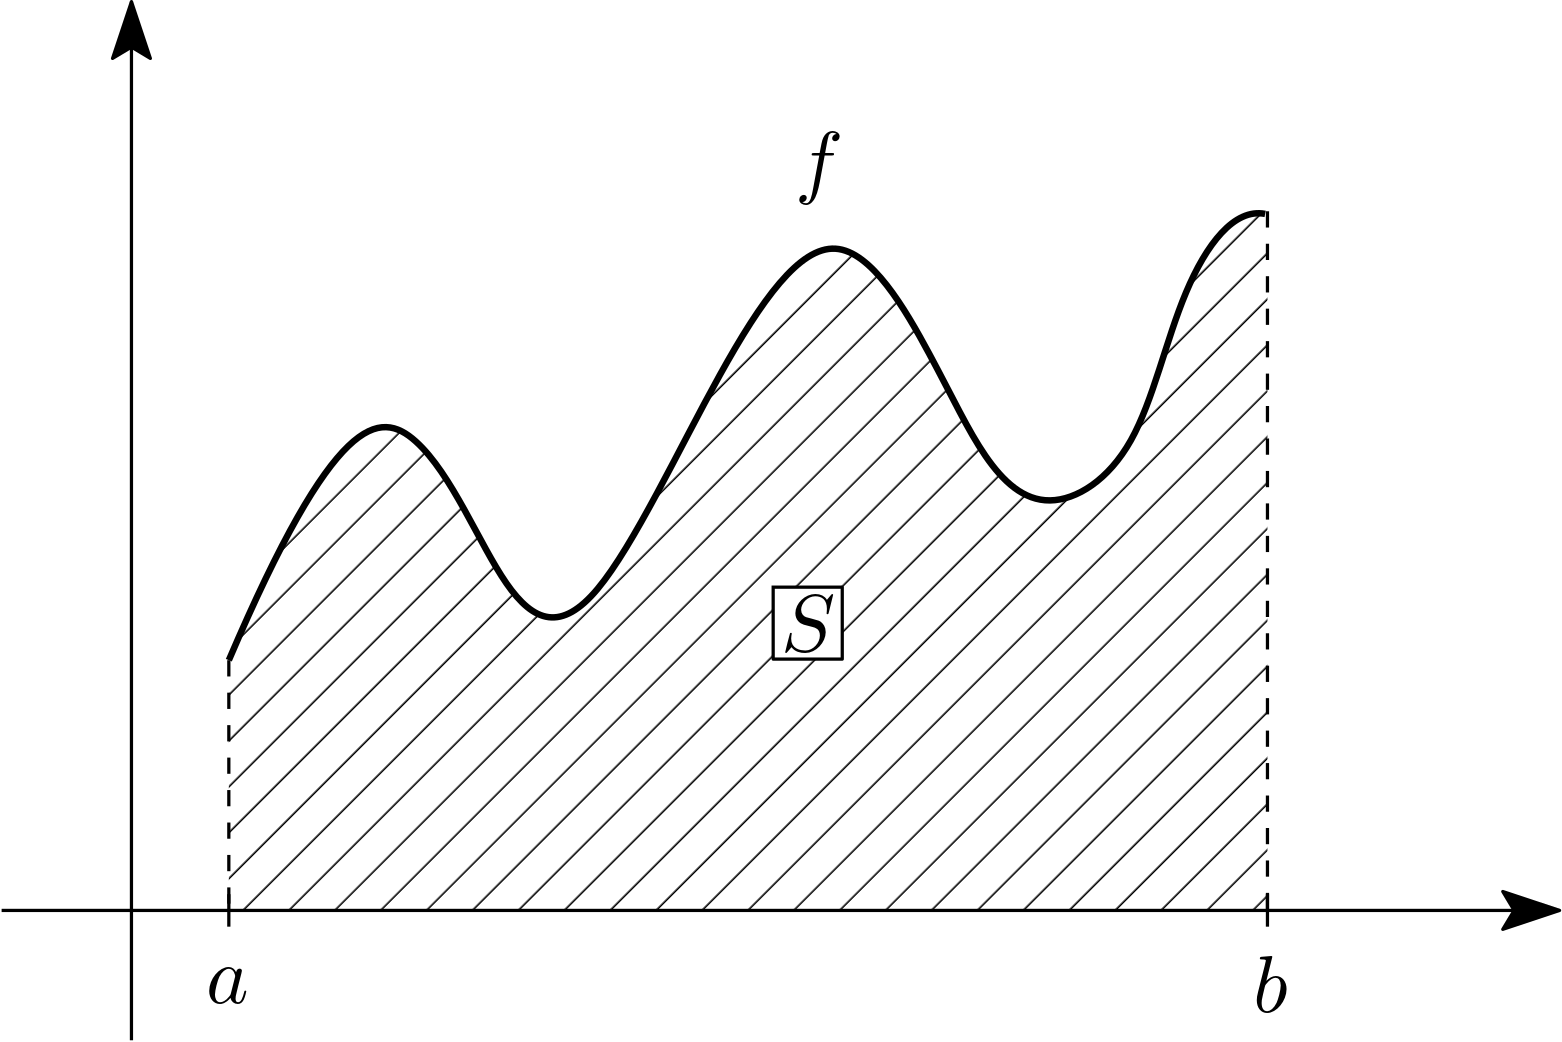
\includegraphics[width=0.35\textwidth]{26_1.png}
	\label{26_1}
	\caption{Интеграл, как площадь под графиком.}
	\label{fig:Площадь под графиком}
\end{figure}
\begin{rem}
	Но ничего конкретного про площадь сказать нельзя, поскольку мы не знаем что такое площадь.
\end{rem}

$2)$ \textbf{Объем тела вращения}: Имеется система координат $Oxy$, функция $f$ над отрезком $[a,b]$, вращаем график вокруг оси $x$.

\begin{figure}[H]
	\centering
	\begin{subfigure}[b]{0.5\textwidth}
		\centering
		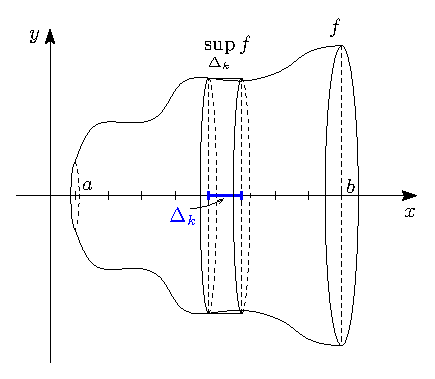
\includegraphics[width=0.8\textwidth]{26_2.eps}
		\label{26_2}
		\caption{Верхний цилиндр.}
	\end{subfigure}
	\begin{subfigure}[b]{0.49\textwidth}
		\centering
		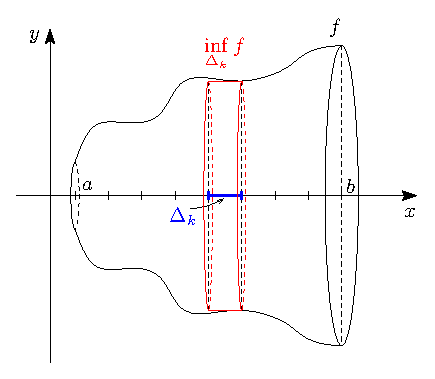
\includegraphics[width=0.82\textwidth]{26_3.eps}
		\caption{Нижний цилиндр.}
		\label{26_3}
	\end{subfigure}
	\caption{Интеграл, как объем тела вращения.}
	\label{fig:Объем тела вращения}
\end{figure}

Хотим найти объем фигуры, полученной вращением $f(x)$ вокруг оси $Ox$. Для этого делим отрезок $[a,b]$, возьмем отрезок $\Delta_k$ и на нём $\sup f(x)$, затем нарисуем цилиндр такого радиуса с центром на оси $x\Rightarrow$	получим внешний цилиндр, если взять $\inf f(x)$, то получим внутренний цилиндр. Значит объем тела вращения $V$ зажимается между следующими суммами:
$$
	\sum\limits_k \left(\inf\limits_{x \smallin \Delta_k}f\right)^2{\cdot}\pi{\cdot}|\Delta_k|	\leq V \leq \sum\limits_k \left(\sup\limits_{x \smallin \Delta_k}f\right)^2{\cdot}\pi{\cdot}|\Delta_k|	
$$
Заметим, что брать квадрат точной верхней/нижней грани у неотрицательной функции  это тоже самое, что и у $f^2$ брать точную верхнюю/нижнюю грань. Тогда:
$$
	\sum\limits_k \left(\inf\limits_{x \smallin \Delta_k}f^2\right){\cdot}\pi{\cdot}|\Delta_k|	\leq V \leq \sum\limits_k \left(\sup\limits_{x \smallin \Delta_k}f^2\right){\cdot}\pi{\cdot}|\Delta_k|
$$
Когда масштаб разбиения $\lambda(\MTB)$ начнет стремиться к нулю, то верхняя/нижняя суммы Дарбу для функции $\pi f^2$ будут стремиться к одному и тому же числу:
$$
	V = \pi {\cdot}\!\ddint{a}{b}f^2(x)dx
$$
\begin{rem}
	Опять же, что такое объем мы пока сказать не можем и выводы сделаны эвристически.
\end{rem} 
\begin{figure}[H]
	\centering
	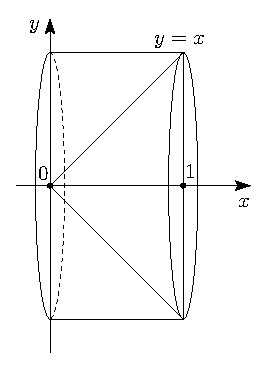
\includegraphics[width=0.25\textwidth]{26_4.eps}
	\label{26_4}
	\caption{Объем конуса/цилиндра.}
	\label{fig:Объем конуса/цилиндра}
\end{figure} 
\textbf{Пример}: Используя формулу выше, можем посчитать объем конуса. Вращаем функцию $y = x$ вокруг оси $Ox$ над отрезком $[0,1]$. Тогда по формуле выше объем будет равен:
$$
	V_{cone} = \pi{\cdot}\!\ddint{0}{1}x^2dx = \dfrac{\pi}{3}
$$
Заметим, если посчитать объем цилиндра, то он будет равен просто $\pi$:
$$
	V_{cyl.} = \pi{\cdot}\! \ddint{0}{1}1{\cdot}dx = \pi
$$
Таким образом, объем конуса составляет одну треть цилиндра. Тут можем обратить внимание на следующий момент: в разрезе одной половины данного цилиндра, площадь треугольника будет занимать ровно половину разреза, как тогда могли получить, что объем конуса не половина? Парадокс в том, что получаем мы не совсем прямоугольники.

$3)$ \textbf{Длина пути}: Пусть есть отображение из $[a,b]$ в $\MR^3 \colon t \mapsto \gamma(t) = (x(t),y(t),z(t))$, где $x(t),y(t), z(t)$ это непрерывно дифференцируемые функции, а $\gamma(t)$ - гладкая кривая. Начиная движение в $a$ и заканчивая в $b$, проезжаем некий путь и спрашивается, какой длины $l$ маршрут мы проехали?
\begin{figure}[H]
	\centering
	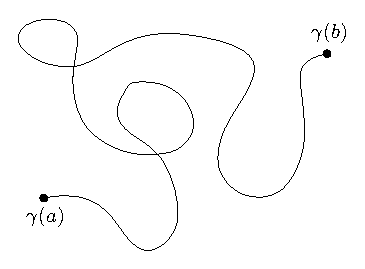
\includegraphics[width=0.30\textwidth]{26_5.eps}
	\label{26_5}
	\caption{Путь из $\gamma(a)$ в $\gamma(b)$.}
	\label{fig:Длина пути}
\end{figure}
Рассуждая немного эвристически, берем отрезок $[a,b]$, делим его, берем отрезок $\Delta_k$. Можем сказать, что весь $l$ складывается из того, что мы прошли на каждом $\Delta_k$: $l_{\Delta_k}$. Эта длина точно не больше, чем движение по прямой с максимальной скоростью и точно не меньше, чем движение по прямой с самой маленькой скоростью за этот же промежуток времени:
$$
	\inf\limits_{\Delta_k}\|\dot{\gamma}\|{\cdot}|\Delta_k| \leq l_{\Delta_k} \leq \sup\limits_{\Delta_k}\|\dot{\gamma}\|{\cdot}|\Delta_k|
$$
Складываем все отрезки и получаем весь путь:
$$
	\sum\limits_k\inf\limits_{\Delta_k}\|\dot{\gamma}\|{\cdot}|\Delta_k| \leq \sum\limits_k l_{\Delta_k} = l \leq \sum\limits_k\sup\limits_{\Delta_k}\|\dot{\gamma}\|{\cdot}|\Delta_k|
$$
Опять же получаем верхнюю и нижнюю суммы Дарбу, тогда в пределе получаем следующее:
$$
	l = \ddint{a}{b}\|\dot{\gamma}(t)\|dt = \ddint{a}{b}\sqrt{\dot{x}^2(t) + \dot{y}^2(t) + \dot{z}^2(t)}dt
$$
\textbf{Пример}: Измерим длину пути на четверти окружности в $\RN{1}$-квадранте. $\gamma(t) = (\cos(t), \sin(t)), \, t \in [0,\tfrac{\pi}{2}]$:
$$
	\ddint{0}{\tfrac{\pi}{2}}\sqrt{(-\sin(t))^2 + (\cos(t))^2}dt  = \ddint{0}{\tfrac{\pi}{2}}1{\cdot}dt = \dfrac{\pi}{2}
$$
Можно взять другую параметризацию: $y = \sqrt{1-x^2} \Rightarrow \gamma(t) = (t,\sqrt{1-t^2}), \, t \in [0,1]$, тогда получим:
$$
	l = \ddint{0}{1}\sqrt{1^2 + \left(\dfrac{-t}{\sqrt{1 - t^2}}\right)^2 }dt = \ddint{0}{1}\dfrac{dt}{\sqrt{1-t^2}}
$$
Но такой интеграл в смысле Римана не существует, поскольку когда подходим к $1$ отношение уходит в бесконечность, а функция для интегрируемости должна быть ограниченной. Чтобы посчитать такой интеграл (ведь мы знаем, что длина у четверти окружности есть), надо немного отойти от $1$:
$$
	\ddint{0}{1-\delta}\dfrac{dt}{\sqrt{1-t^2}} = \arcsin(1-\delta) - \arcsin(0) = \arcsin(1-\delta) \xrightarrow[\delta \to 0]{} \arcsin(1) = \dfrac{\pi}{2}
$$
В таких случаях предлагается понимать интегралы с функциями, которые уходят на бесконечность в отдельных точках, как пределы, отступив от особенностей:
$$
	\ddint{0}{1}\dfrac{dt}{\sqrt{1-t^2}} = \lim\limits_{\delta \to 0} \ddint{0}{1 - \delta}\dfrac{dt}{\sqrt{1-t^2}}
$$
Тогда говорят, что рассматриваем \uwave{несобственный интеграл Римана}.
\end{document}